% ---------
% --------
%!TEX TS-program = pdflatex
%!TEX encoding = UTF-8 Unicode
%!TEX spellcheck = English (Aspell)

\documentclass[11pt]{article}
\usepackage{jeffe,handout,graphicx,varwidth}
\usepackage{fourier-orns}
\usepackage{mathtools}
\usepackage[normalem]{ulem} % either use this (simple) or
\usepackage{tikz}


\def\Sym#1{\texttt{\color{BrickRed}#1}}
\allowdisplaybreaks

\begin{document}

\begin{center}
\Large\textbf{CSCI 432/532, Spring 2026}%
\\
\LARGE\textbf{Homework 8}%
\\[0.5ex]
\large Due Monday, March 16 at 8:30am
\end{center}

\bigskip
\hrule
\bigskip

\subsection*{Submission Requirements}
\begin{itemize}
    \item Type or clearly hand-write your solutions into a PDF format so that they are legible and professional. Submit your PDF on Canvas or Gradescope. 
	\item Put each \textbf{sub}problem on a separate page and select the corresponding problem via the Gradescope interface.
    \item Do not submit your first draft. Type or clearly re-write your solutions for your final submission. If your submission is not legible, we will ask you to resubmit.
\end{itemize}

\subsection*{Collaboration and Resources}

The \emph{best} resources for completing the homework are (in no particular order):
\begin{itemize}
	\item Your own notes from lectures and problem sessions, and/or lecture recordings.
	\item The lecture notes linked from the course website for the lecture day.
	\item The questions channel on Discord.
	\item Office hours.
	\item Discussions with classmates.
\end{itemize}
You may also access almost any resource in preparing your solution to the
homework. The exception is that you may not seek answers to the problems on the
homework directly, such as by pasting them into a GenAI tool, searching for
solutions on a search engine, looking for them on Chegg or similar websites, or
asking another person for the solution.

Additionally, you \EMPH{must}
\begin{itemize}
    \item Write your solutions in your own words---this means that you should never be \emph{copying}
    anything of substance from any source, and
    \item credit every resource you use, including GenAI tools, by providing links or full chat transcripts.
    If you use the provided LaTeX template, you can use the \texttt{Sources}
    environment for this. Ask if you need help!
\end{itemize}


\begin{boxquote}{0.9}
Remember, if you choose to use GenAI tools, not only must you provide a full
transcript of your conversation (or a link to one), you must also use the
following prompt (or some variation of it), and provide a full transcript of
the conversation.
\end{boxquote}  

Prompt:
\begin{boxquote}{0.9}
You are acting as a teaching assistant for an advanced undergraduate/graduate
algorithms and computer science theory course.

Your role is not to provide full solutions or final answers.

Instead, you should act like we are having a conversation. Ask me a single
question and let me respond. Avoid asking me many questions at once or giving
me a lot of information at one time. Guide me using hints, leading questions,
partial insights, and sanity checks.  Help me debug my own proofs, algorithms,
or reductions. Do not give a complete solution or full proofs. Be patient with
me. Don't give me details so that I can move on to the next part of a problem.
Make sure that I understood before moving on.

The course uses Jeff Erickson's Models of Computation lecture notes, so you should
guide me to answer problems using the definitions, notation, and style from those notes.

Assume I am a serious student trying to learn, not to shortcut the assignment.
I am attaching the assignment, so you should refuse to provide a complete solution
to the problems listed. Of course, you can walk me through the "Solved
Problems" listed at the end if I ask.
\end{boxquote}  

\newpage
%----------------------------------------------------------------------

\headers{CSCI 432/532}{Homework 8 (due March 16)}{Spring 2026}

\noindent \Hint{Make sure you understand the definitions of the problems you are trying to prove NP-hard.
Only a small amount of partial credit will be given for submissions that do not address the correct
computational problems.}

Rubric for both of the following:

\begin{Rubric}{Standard NP-hardness rubric}~
10 points = 
\begin{itemize}
\item[+]
1 point for choosing a reasonable NP-hard problem X to reduce from.
\begin{itemize}\cramped
\item
The Cook-Levin theorem implies that \emph{in principle} one can prove NP-hardness by reduction from \emph{any} NP-complete problem.  What we’re looking for here is a problem where a simple and direct NP-hardness proof seems likely.
\item
You can use any of the NP-hard problems listed in the lecture notes (except the one you are trying to prove NP-hard, of course).
\end{itemize}

\item[+]
2 points for a \emph{structurally sound} polynomial-time reduction.  Specifically, the reduction must:
\begin{itemize}\cramped
\item take an \emph{arbitrary} instance of the declared problem X \EMPH{and nothing else} as input,
\item transform that input into a corresponding instance of Y (the problem we’re trying to prove NP-hard), 
\item transform the output of the oracle for Y into a reasonable output for X, and
\item run in polynomial time.
\end{itemize}
(The output transformation is usually trivial.)  This is strictly about the structure of the reduction algorithm, not about its correctness.  No credit for the rest of the problem if this is wrong.

\item[+] 2 points for a \emph{correct} polynomial-time reduction.  That is, assuming a black-box algorithm that solves Y in polynomial time, the proposed reduction actually solves problem X in polynomial time.
\item[+] 2 points for the “if” proof of correctness.  (Every good instance of X is transformed into a good instance of Y.)
\item[+] 2 points for the “only if” proof of correctness.  (Every bad instance of X is transformed into a bad instance of Y.)
\item[+] 1 point for writing “polynomial time”
\medskip
\item
An incorrect but structurally sound polynomial-time reduction that still satisfies half of the correctness proof is worth at most 5/10 (= 1 for reasonable reduction source + 2 for structural soundness + 2 for half of the proof)
\item
A reduction in the wrong direction is worth at most 1/10 (for choosing a reasonable problem)
\end{itemize}
\end{Rubric}

%----------------------------------------------------------------------
\begin{enumerate}


\item
A \emph{lollipop} of size $\ell$ is an undirected graph consisting of a (simple)
cycle of length $\ell$ and a (simple) path of length $\ell$, where one endpoint
of the path lies on the cycle, and otherwise the cycle and the path are
disjoint.  Every lollipop of size $\ell$ has exactly $2\ell$ vertices and $2\ell$
edges.  For example, the $4\times 4$ grid graph shown below contains a lollipop
subgraph of size~$8$.

\begin{center}
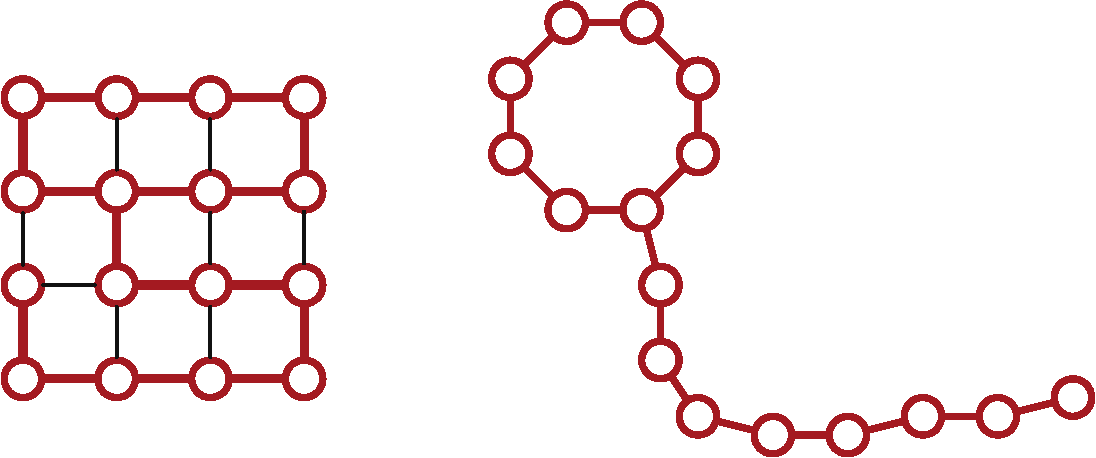
\includegraphics[scale=0.4]{../Fig/6-lollipop}
\end{center}
Prove that it is NP-hard to find the size of the the largest lollipop subgraph of a given undirected graph.


%----------------------------------------------------------------------


\item
Recall that a \emph{3-coloring} of a graph assigns each vertex one of three colors, say red, yellow, and blue.  A 3-coloring is \emph{proper} if every edge has endpoints with different colors.  The \textsc{3Color} problem asks, given an arbitrary undirected graph $G$, whether $G$ has a proper 3-coloring.

Call a 3-coloring of a graph $G$ \emph{almost 3-coloring} if each vertex has \emph{at most one neighbor} with the same color.  The \textsc{Almost3Color} problem asks, given an arbitrary undirected graph $G$, whether $G$ has a almost 3-coloring.

\begin{center}
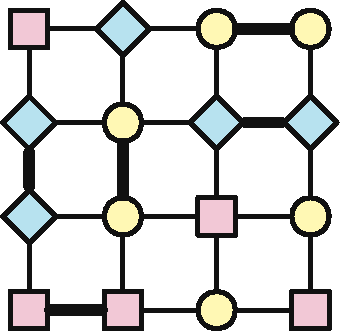
\includegraphics[scale=0.4]{../Fig/3-quasi-coloring}
\end{center}

\begin{enumerate}\itemsep2ex
\item
Consider the following attempt to prove that \textsc{Almost3Color} is NP-hard, using a reduction from \textsc{3Color}.

\begin{Solution}
We reduce from \textsc{3Color}.  Given an arbitrary input graph $G$, we
construct a new graph $H$ by attaching a clique of 4 vertices to every vertex
of~$G$.  Specifically, for each vertex $v$ in $G$, the graph $H$ contains three
new vertices $v_1, v_2, v_3$, along with edges $vv_1, vv_2, vv_3, v_1v_2,
v_1v_3, v_2v_3$. I claim that
\begin{center}
\fbox{
	\begin{varwidth}{\textwidth}
		\centering
			$G$ has a proper 3-coloring\\
			if and only if\\
			$H$ has an almost 3-coloring.
	\end{varwidth}
}
\end{center}
\begin{itemize}
\item[$\Longrightarrow$]
Suppose $G$ has a proper 3-coloring, using the colors red, yellow, and blue.
Extend this color assignment to the vertices of $H$ by coloring each
vertex~$v_1$ red, each vertex $v_2$ yellow, and each vertex $v_3$ blue.  With
this assignment, each vertex of $H$ has at most one neighbor with the same
color.  Specifically, each vertex of $G$ has the same color as one of the
vertices in its gadget, and the other two vertices in $v$’s gadget have no
neighbors with the same color.

\item[$\rlap{\quad\slash}\rlap{\quad\textbackslash}\Longleftarrow$] Now suppose $H$ has an almost 3-coloring.  Then $G$ must have a proper 3-coloring because\dots um\dots 
\end{itemize}
\end{Solution}

Describe a graph $G$ that does not have a proper 3-coloring, such that the graph $H$ constructed by this reduction does have an almost 3-coloring.

\item
Describe a small graph $X$ with the following property: In every almost 3-coloring of $X$, every vertex of $X$ has \emph{exactly} one neighbor with the same color. [Hint: make sure you
understand what this problem is asking for. You need to ask yourself: for \emph{every possible} almost 3-coloring of $X$, does every vertex have exactly one neighbor with the same color?
It is not sufficient for \emph{some} almost 3-coloring of $X$ to have this property.]

\item
Describe a correct polynomial-time reduction from \textsc{3Color} to \textsc{Almost\-3Color}.  \Hint{Use your graph from part (b) as a gadget.}  This reduction will prove that \textsc{Almost3Color} is indeed NP-hard.

\end{enumerate}

%----------------------------------------------------------------------
\end{enumerate}

% ----------------------------------------------------------------------
\newpage
\subsection*{Solved Problem}


\begin{enumerate}\parindent1.5em
\item[3.]
A \emph{double-Hamiltonian tour} in an undirected graph $G$ is a closed walk that visits every vertex in $G$ exactly twice.  Prove that it is NP-hard to decide whether a given graph $G$ has a double-Hamiltonian tour.

\begin{center}
\footnotesize\sffamily
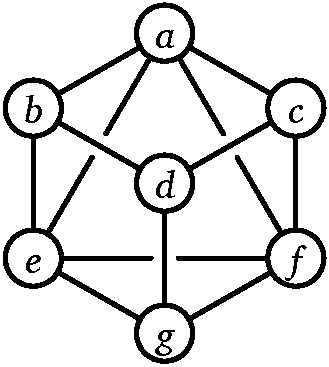
\includegraphics[scale=0.4]{../Fig/doubleham-example}\\
This graph contains the double-Hamiltonian tour $a\arcto b\arcto d\arcto g\arcto e\arcto b\arcto d\arcto c\arcto f\arcto a\arcto c\arcto f\arcto g\arcto e\arcto a$.
\end{center}

\begin{Solution}
We prove the problem is {NP}-hard with a reduction from the standard Hamiltonian cycle problem.  Let $G$ be an arbitrary undirected graph.  We construct a new graph $H$ by attaching a small gadget to every vertex of $G$.  Specifically, for each vertex $v$, we add two vertices $v^\sharp$ and~$v^\flat$, along with three edges $vv^\flat$, $vv^\sharp$, and $v^\flat v^\sharp$.

\begin{center}\footnotesize\sffamily
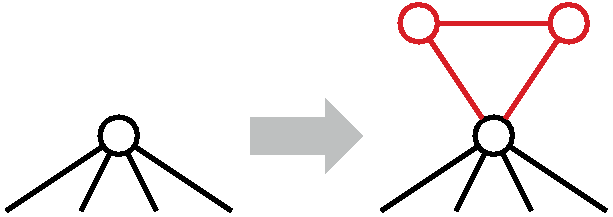
\includegraphics[scale=0.4]{../Fig/double-Ham-reduction}\\
A vertex in $G$ and the corresponding vertex gadget in $H$.
\end{center}
\unskip
Now I claim that
\begin{center}
\fbox{
	\begin{varwidth}{\textwidth}
		\centering
			$G$ has a Hamiltonian cycle\\
			if and only if\\
			$H$ has a double-Hamiltonian tour.
	\end{varwidth}
}
\end{center}

\begin{itemize}
\item[$\Longrightarrow$]
Suppose $G$ contains a Hamiltonian cycle $C = \arc{\arc{\arc{v_1}{v_2}}{\cdots}}{\arc{v_n}{v_1}}$.  We can construct a double-Hamiltonian tour of $H$ by replacing each vertex $v_i$ in $C$ with the following walk:
\[
	\arc{\arc{\arc{\cdots}{v_i}}
			{\arc{v_i^\flat}{v_i^\sharp}}}
		{\arc{\arc{v_i^\flat}{v_i^\sharp}}
			{\arc{v_i}{\cdots}}}
\]

\item[$\Longleftarrow$]
Conversely, suppose $H$ has a double-Hamiltonian tour $D$.  Consider any vertex $v$ in the original graph $G$; the tour $D$ must visit $v$ exactly twice.  Those two visits split $D$ into two closed walks, each of which visits $v$ exactly once.  Any walk from~$v^\flat$ or~$v^\sharp$ to any other vertex in $H$ must pass through $v$.  Thus, one of the two closed walks visits only the vertices~$v$,~$v^\flat$, and $v^\sharp$.  Thus, if we remove the vertices and edges in $H\setminus G$ from~$D$, we obtain a closed walk in~$G$ that visits every vertex in~$G$ exactly once.
\end{itemize}

\noindent
Given any graph $G$, we can clearly construct the corresponding graph $H$ in polynomial time by brute force.

\bigskip
\hrule
\medskip

With more effort, we can construct a graph $H$ that contains a double-Hamiltonian tour \EMPH{that traverses each edge of $H$ at most once} if and only if $G$ contains a Hamiltonian cycle.  For each vertex $v$ in $G$ we attach a more complex gadget containing five vertices and eleven edges, as shown on the next page.

\begin{center}\footnotesize\sffamily
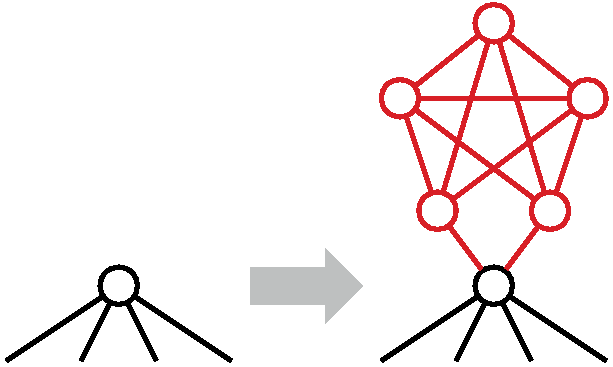
\includegraphics[scale=0.4]{../Fig/double-Ham-reduction2}\\
A vertex in $G$, and the corresponding modified vertex gadget in $H$.
\end{center}
\unskip
\end{Solution}
\unskip

\begin{rubric}
10 points, standard polynomial-time reduction rubric.  This is not the only correct solution.
\end{rubric}

\begin{Solution}[self-loops]
We attempt to prove the problem is {NP}-hard with a reduction from the Hamiltonian cycle problem.  Let $G$ be an arbitrary undirected graph.  We construct a new graph $H$ by attaching a self-loop every vertex of $G$.  Given any graph $G$, we can clearly construct the corresponding graph $H$ in polynomial time.

\begin{center}\footnotesize\sffamily
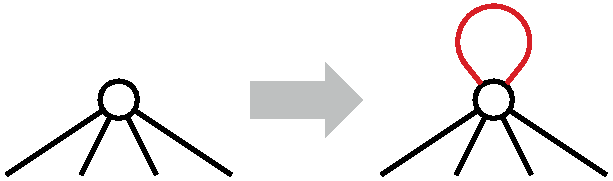
\includegraphics[scale=0.4]{../Fig/double-Ham-reduction0}\\
An incorrect vertex gadget.
\end{center}
\unskip
Now I claim that
\begin{center}
\fbox{
	\begin{varwidth}{\textwidth}
		\centering
			$G$ has a Hamiltonian cycle\\
			if and only if\\
			$H$ has a double-Hamiltonian tour.
	\end{varwidth}
}
\end{center}

\begin{itemize}
\item[$\Longrightarrow$]

Suppose $G$ has a Hamiltonian cycle
$\arc{\arc{\arc{v_1}{v_2}}{\cdots}}{\arc{v_n}{v_1}}$.  We can construct a
double-Hamiltonian tour of $H$ by alternating between edges of the Hamiltonian
cycle and self-loops:
\(
	v_1 \arcto v_1 \arcto v_2 \arcto v_2 \arcto v_3 \arcto \cdots \arcto v_n \arcto v_n \arcto v_1.
\)

\item[$\rlap{\quad\slash}\rlap{\quad\textbackslash}\Longleftarrow$]
Um\dots
\end{itemize}
\unskip
Unfortunately, if $H$ has a double-Hamiltonian tour, we \emph{cannot} conclude that~$G$ has a Hamiltonian cycle, because we cannot guarantee that a double-Hamiltonian tour in $H$ uses \emph{any} self-loops.  The graph $G$ shown below is a counterexample; it has a double-Hamiltonian tour (even before adding self-loops!\@) but no Hamiltonian cycle. 

\begin{center}\footnotesize\sffamily
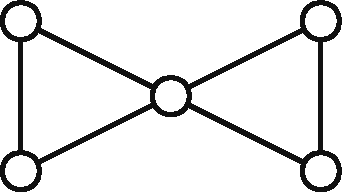
\includegraphics[scale=0.4]{../Fig/doubleham}\\
This graph has a double-Hamiltonian tour.
\end{center}
\unskip
\end{Solution}

\end{enumerate}


\newpage
\begin{Rubric}{Some useful NP-hard problems}
You are welcome to use any of these in your own NP-hardness proofs, except of course for the specific problem you are trying to prove NP-hard.

\begin{description}
\item[\mathsc{CircuitSat}:]
Given a boolean circuit, are there any input values that make the circuit output \mathsc{\textrm{True}}?

\item[\mathsc{3Sat}:]
Given a boolean formula in conjunctive normal form, with exactly three distinct literals per clause, does the formula have a satisfying assignment?

\item[\mathsc{MaxIndependentSet}:]
Given an undirected graph $G$, what is the size of the largest subset of vertices in $G$ that have no edges among them?

\item[\mathsc{MaxClique}:]
Given an undirected graph $G$, what is the size of the largest complete subgraph of $G$?

\item[\mathsc{Min\-Vertex\-Cover}:]
Given an undirected graph $G$, what is the size of the smallest subset of vertices that touch every edge in~$G$?

\item[\mathsc{MinSetCover}:]
Given a collection of subsets $S_1, S_2, \dots, S_m$ of a set $S$, what is the size of the smallest subcollection whose union is $S$?

\item[\mathsc{MinHittingSet}:]
Given a collection of subsets $S_1, S_2, \dots, S_m$ of a set $S$, what is the size of the smallest subset of $S$ that intersects every subset $S_i$?

\item[\mathsc{3Color}:]
Given an undirected graph $G$, can its vertices be colored with three colors, so that every edge touches vertices with two different colors?

\item[\mathsc{ChromaticNumber}:]
Given an undirected graph $G$, what is the minimum number of colors required to color its vertices, so that every edge touches vertices with two different colors?

\item[\mathsc{HamiltonianPath}:]
Given graph $G$ (either directed or undirected), is there a path in $G$ that visits every vertex exactly once?

\item[\mathsc{HamiltonianCycle}:]
Given a graph $G$ (either directed or undirected), is there a cycle in $G$ that visits every vertex exactly once?

\item[\mathsc{TravelingSalesman}:]
Given a graph $G$ (either directed or undirected) with weighted edges, what is the minimum total weight of any Hamiltonian path/cycle in $G$?

\item[\mathsc{LongestPath}:]
Given a graph $G$ (either directed or undirected, possibly with weighted edges), what is the length of the longest simple path in $G$?

\item[\mathsc{SteinerTree}:]  Given an undirected graph $G$ with some of the vertices marked, what is the minimum number of edges in a subtree of $G$ that contains every marked vertex? 

\item[\mathsc{SubsetSum}:]
Given a set $X$ of positive integers and an integer $k$, does $X$ have a subset whose elements sum to $k$?

\item[\mathsc{Partition}:]
Given a set $X$ of positive integers, can $X$ be partitioned into two subsets with the same sum?

\item[\mathsc{3Partition}:]
Given a set $X$ of $3n$ positive integers, can $X$ be partitioned into $n$ three-element subsets, all with the same sum?

\item[\mathsc{IntegerLinearProgramming}:]
Given a matrix $A\in\Z^{n\times d}$ and two vectors $b\in\Z^n$ and $c\in Z^d$, compute  $\max\set{c\cdot x\mid Ax\le b, x\ge 0, x\in\Z^d}$.

\item[\mathsc{FeasibleILP}:]
Given a matrix $A\in\Z^{n\times d}$ and a vector $b\in\Z^n$, determine whether the set of feasible integer points $\max\set{x\in\Z^d\mid Ax\le b, x\ge 0}$ is empty.

\item[\mathsc{Draughts}:]
Given an $n\times n$ international draughts configuration, what is the largest number of pieces that can (and therefore must) be captured in a single move?

\item[\mathsc{SuperMarioBrothers}:]
Given an $n\times n$ Super Mario Brothers level, can Mario reach the castle?

\end{description}
\end{Rubric}

%----------------------------------------------------------------------



\end{document}
